\documentclass[11pt]{article}

%Don't change any thing before \begin{document}
%They are not useful for now, but later when you try to add figures
%these might be useful. In fact if you use sth fancy, you might need
%to add more packages, or macros.
\usepackage{amssymb,amsmath}
\usepackage{times,psfrag,epsf,epsfig,graphics,graphicx}
\usepackage{algorithm}
\usepackage{algorithmic}

\begin{document}
\date{}

\title{CSCI 246: Assignment~5~(6 points)}

\author{William Jardee}

\maketitle

 
\section*{Problem 1.}

\noindent
You have two parents, four grandparents, eight great-grandparents, and so forth.
\newline

\noindent
(1.1) If all your ancestors were distinct, what would be the total number of your ancestors for the past 41 generations (counting your parents' generation as the first generation)?
\newline

$2^{41} = 2.99 \times 10^{12}$\\

\newline

\noindent
(1.2) Assuming that each generation represents 25 years, how long (in years) is 41 generation?
\newline

$t = 25 \cdot 2^{41} = 5.498 \times 10^{13}$\\

\newline

\noindent
(1.3) The total number of people who have ever lived is approximately 10
billion, which is $10^{10}$. Compare this fact to (1.1), what can you deduce
about the family tree rooted at you?
\newline

The number I got is 100 times larger than possible. So, something about the original statement is false. Most likely, the statement falls apart at the idea that my ancestors are distinct. If, after 5 generations, branches of the tree started crossing then the number would be cut down drastically. If we know for sure that all the ancestors are distinct, then the depth must be wrong. If the depth was around $2^{33}$ (33 generations), then the number of ancestors is about $10^{10}$.

\newpage


\section*{Problem 2.}

\noindent
A polygon is {\em convex} means that given any two points on or inside the polygon, the segment joining the points lie entirely in the polygon.
Use mathematical induction to prove that for every integer $n\geq 3$, the interior angles of any $n$-sided convex polygon add up to $180\cdot (n-2)$ degrees.
\newline

{\bf Proof by Induction:}

Let us take the base case of a convex triangle (this is any triangle). It is simple enough to show that the sum of the angles of this polygon is $180$. If we count $n$ as the number of sides, then $n=3$. So we see that the equation $180(n-2)$ works to describe the total sum of degree of angles for $n=3$.\\

It is beyond the scope of this proof to prove this fact, so we will use it without anything base intuitive justification.If we want to create a new side on a polygon we can split an existing side into two new sides. This will create a shape of the original polygon with a triangle attached to it. The total sum of this new polygon will be the sum of the angles of this original polygon and this new triangle. The picture below describes this idea: 
\begin{center}
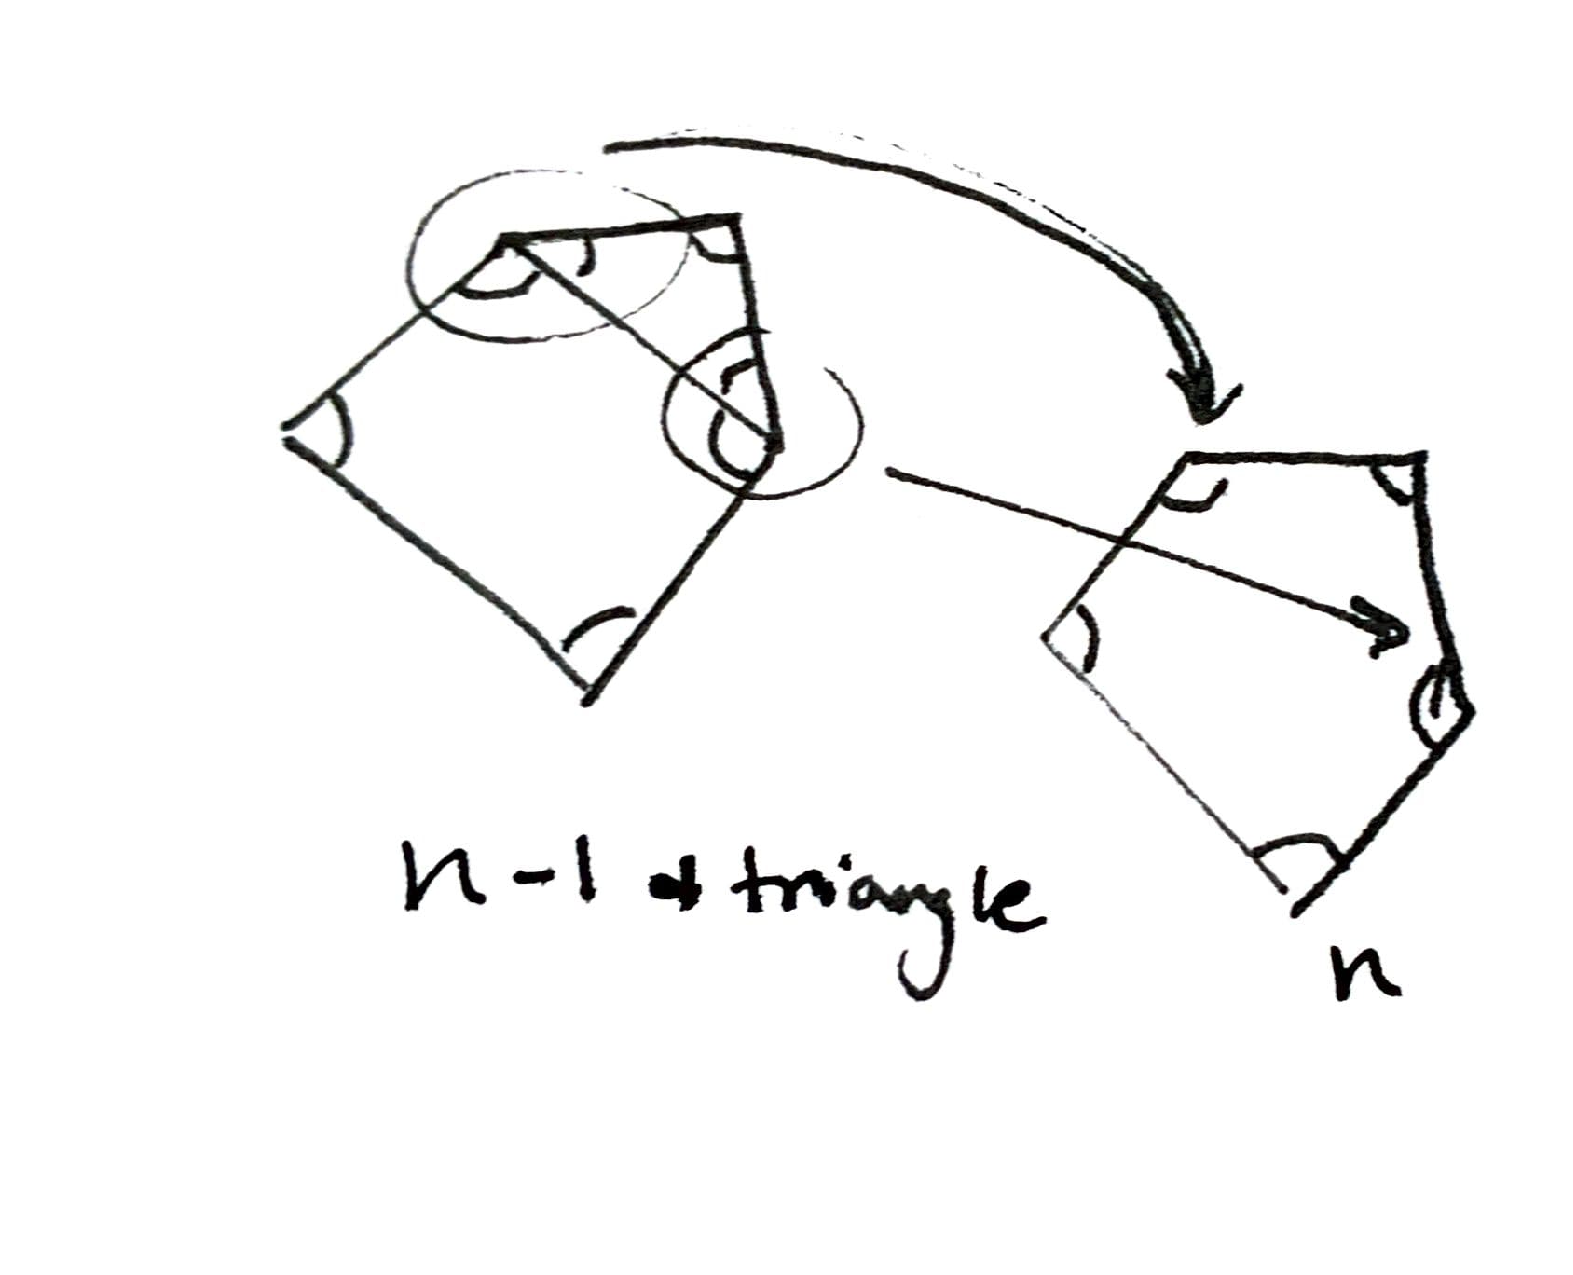
\includegraphics[width = 150]{Homework/Scan Oct 20, 2020.pdf}
\end{center}
With that basis and the base case already dealt with, let's do the inductive step:\\

Assume that we have a polygon with k sides, such that $k\geq 3$, and the total sum of interior angles can be written as $180\cdot (k-2)$. If we pull one of the sides into two (as above), then we now have a polygon with $k+1$ sides. The total sum of interior angles can be written as $180\cdot (k-2) + 180$, since a triangle's angles have a sum of 180. $180 \cdot (k-2) + 180 = 180 \cdot ((k+1)-2)$. Thus, through inductive reasoning, the equation $180\cdot (n-2)$ must describe the sum of interior angles for polygons with as many or more sides than a triangle, or $n\geq 3$.
\begin{flushright}$\blacksquare$\end{flushright}




\newpage

\section*{Problem 3.}

The given sequence is defined recursively. Using (directed) iteration to solve it, simplify your answer if possible.

$t_k=t_{k-1}+3k+1$, for each integer $k\geq 1$,

$t_0=0$.
\newline

What is $t_n$=?\\

Showing the process I went through:\\
$t_1 = 3 + 1$\\
$t_2 = (3+1)+(3 \cdot 2 +1) = 3(1+2) +2(1)$\\
$t_3 = (3+1)+(3 \cdot 2 +1) + (3 \cdot 3 +1) = 3(1+2+3) + 3(1)$\\

So, by studying the pattern, it follows that:
\[t_n = 3 \Big(\sum\limits^n_{i=1} n\Big) +n = \frac{n(n+1)}{2} + n = \boxed{\frac{n(n+3)}{2}}\]

\newpage

\noindent
\section*{Problem 4.}

Let $T(n)$ be the running time (in \# of steps) of Peter's program, where $n$ is the input size $n$.
Solve the following recurrence relation and prove your claim by induction.\\
$T(n)=2T(n/2)+n^2$,\\
$T(1)=1$.
\newline

\noindent
\begin{center}

$T(n) = 2T(\frac{n}{2}) + n^2$\\
$T(n) = 2(2T(\frac{n}{2^2}) + (\frac{n}{2})^2) +n^2$\\
$T(n) = 4T(\frac{n}{2^2}) + (\frac{n^2}{2}) +n^2$\\
$T(n) = 4(2T(\frac{n}{2^3} + (\frac{n}{2^2})^2)+\frac{n^2}{2} + n^2$\\
$T(n) = 8T(\frac{n}{2^3}) + \frac{n^2}{4} + \frac{n^2}{2} + n^2$\\
$T(n) = 2^i T(\frac{n}{2^i}) + \frac{2^i -1}{2^{i-1}}n^2$
\end{center}

Now suppose $2^i = n$, or $i = \log_2(n)$

\begin{center}
    $T(n) = 2^{\log_2(n)} T(1) + \frac{2^{\log_2(n)} - 1}{2^{\log_2(n)-1}}n^2$\\
    $T(n) = nT(1) + \frac{n-1}{\frac{1}{2}n}n^2 = nT(1) + \frac{2(n-1)}{n}n^2$
    $T(n) = n + 2(n-1)n = n(2n -1)$
\end{center}

So we get that $\boxed{T(n) = n(2n-1)}$\\

{\bf Proof by Induction:}\\

Base case: $n=1$\\
$T(1) = 1(2-1)=1$. So the equation holds for the $n=1$ step\\

Inductive Step: Let us assume that the $k$ case works, and consequently all the values less than k work as well, where $k\geq 1$\\
$T(k+1) = 2T(\frac{k+1}{2}) + (k+1)^2 = 2((\frac{k+1}{2})(2(\frac{k+1}{2})-1)+(k+1)^2$\\
$T(k+1) = (k+1)(k+1-1) + (k+1)(k+1) = (k+1)(k) + (k+1)(k+1)$\\
$T(k+1) = (k+1)(2k+1) = (k+1)(2k+2 -1) = (k+1)(2(k+1) -1)$\\

We see that this is in the format for the proposed solution $T(n) = n(2n-1)$. So if the equation holds for the $k$ case, as it does in our base case, than any value greater than $k$ also follows the pattern. Thus we can write $\boxed{T(n) = n(2n-1)}$ for $n\geq 1$.
\begin{flushright}$\blacksquare$\end{flushright}


\newpage


\section*{Problem 5.}

Let $T(n)$ be the running time (in \# of steps) of Sam's program, where $n$ is the input size $n$.
Solve the following recurrence relation and prove your claim by induction.
\newline

$T(n)=4T(n/2)+n^2$,

$T(1)=1$.
\newline
\newline
\noindent
    $T(n) = 4(T(\frac{n}{2})+n^2 = 4(4T(\frac{n}{2^2}) + (\frac{n}{2})^2) +n^2$\\
    $T(n) = 16T(\frac{n}{2^2}) + n^2 + n^2$\\
    $T(n)=16((4T(\frac{n}{2^3})+(\frac{n}{2^2})^2 + 2n^2)$\\
    $T(n)= 64T(\frac{n}{2^3}) + 3n^2$\\
    $T(n)= 4^i T(\frac{n}{2^i}) + i\cdot n^2$\\\\
We know the deal, $i = \log_2(n)$\\\\
$T(n) = 4^{\log_2(n)} T(1) + \log_2(n)\cdotn^2$\\
$T(n) = n^2 + n^2 \cdot \log_2(n) = n^2(1+\log_2(n))$\\

$\boxed{T(n) = n^2(1+\log_2(n))}$\\\\

{\bf Proof by Induction:}\\
Base case: $n=1$\\
$T(1) = 1(1+\log_2(1)) = 1$. So the base case of $n=1$ holds.\\

Inductive Step:\\
Let us assume that k holds such that $k\geq 1$, and all the $n < k$ hold as well.\\
$T(k+1) = 4T(\frac{k+1}{2}) + (k+1)^2$\\
$T(k+1) = 4((\frac{k+1}{2})^2(1+\log_2(\frac{k+1}{2})))+(k+1)^2$\\
$T(k+1) = (k+1)^2(1+\log_2(k+1) - \log_2(2)) + (k+1)^2$\\
$T(k+1) = (k+1)^2(\log_2(k+1))+(k+1)^2$\\
$T(k+1) = (k+1)^2(1+ \log_2(k+1))$\\

We can see that if the $k$ case, and all cases below it, hold then the $k+1$ case turns into the form of $T(n) = n^2(1+\log(n))$. Thus we can say, by induction that $\boxed{T(n) = n^2(1+\log(n))}$ for all $n \geq 1$.
\begin{flushright}$\blacksquare$\end{flushright}


\end{document}
